\subsection{Les classes agents}
\begin{frame}
\frametitle{Modèle}
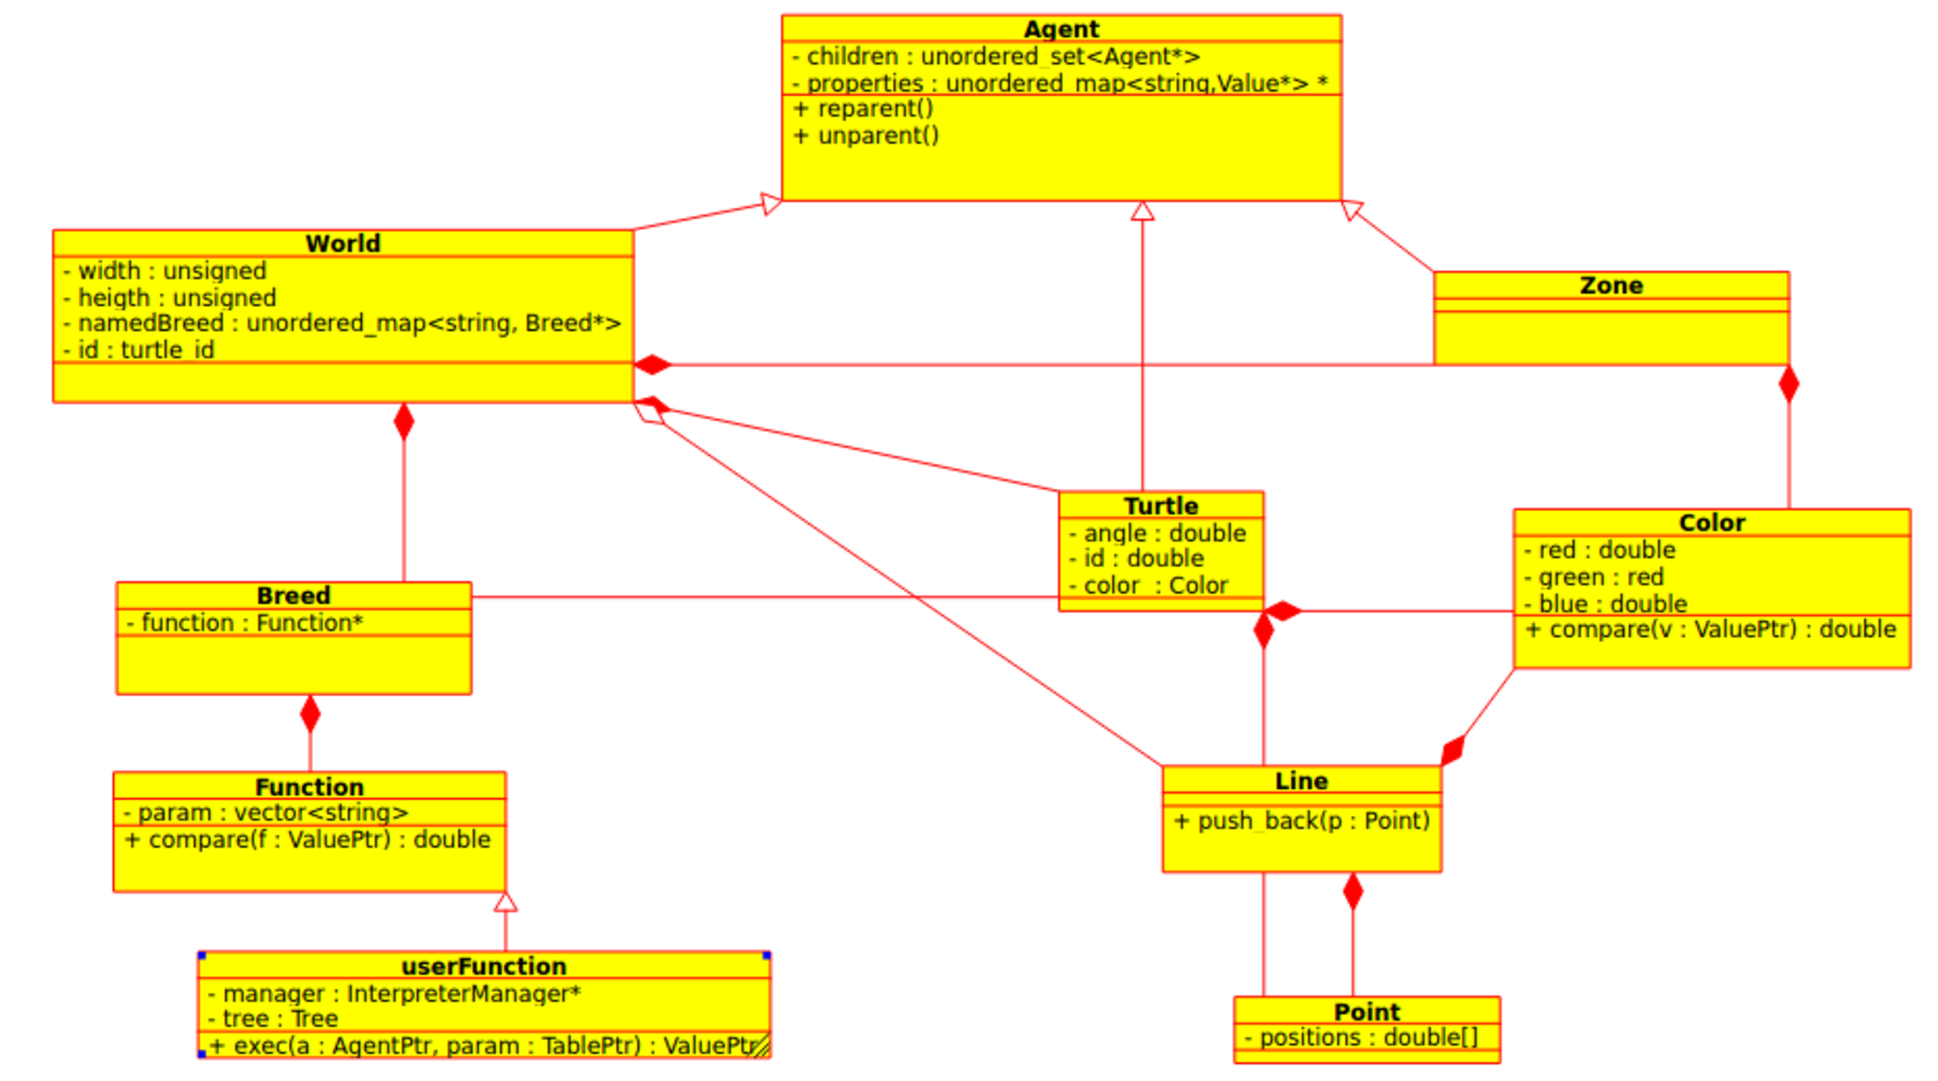
\includegraphics[scale=0.31]{doc/Presentation/image/agents.pdf}
\end{frame}

\note{diagramme=modèle à l'état final.\\
Sprint 1 : turtle point, line, world. Détail...\\
Sprint 2 : classes agent(regroupe comportement) et breed(nommée ou pas), ajout des fonctions, qui stocke un arbre abstrait, contenant le code de la fonction déjà analysé.; Détail....\\
Sprint 3 : les communications : zones propriétés et tortues send, recv...\\
 			export : méthode dans chaque agent\\
 			ajout user function
}

\subsection{Les types}
\begin{frame}
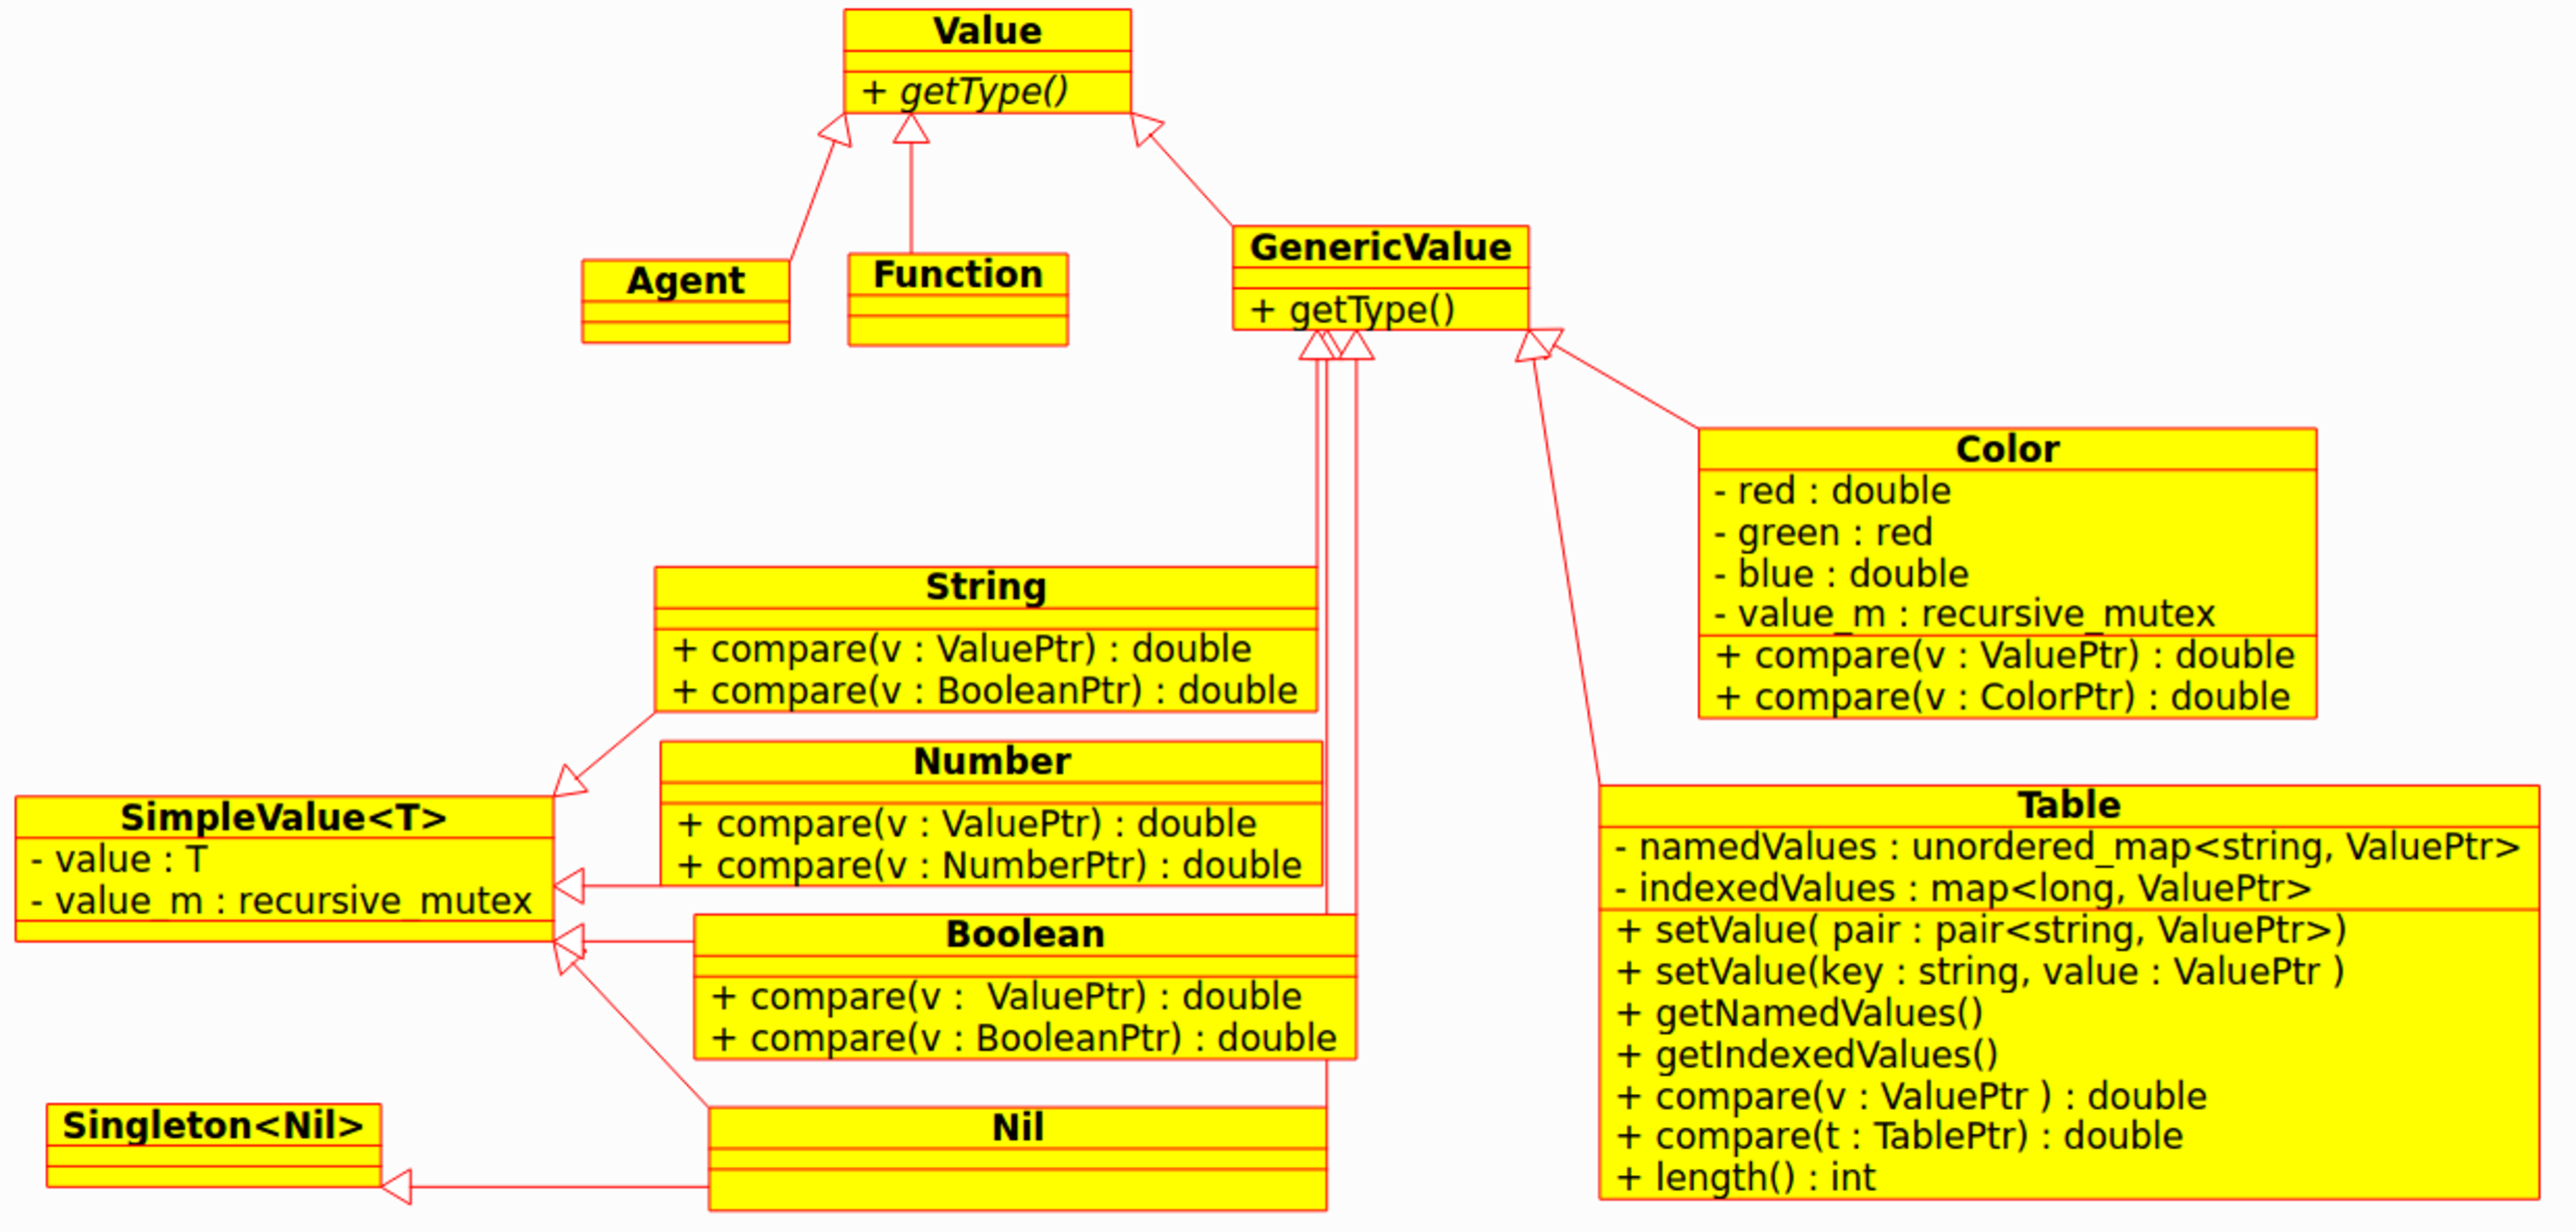
\includegraphics[scale=0.27]{doc/Presentation/image/types.pdf}
\end{frame}
\note{1er sprint : color nil et value\\
2eme : compléxifié avec simple value pour les mutexs\\
4eme : table et mutex recursifs
}
